\documentclass[12pt, a4paper, english]{report}

\usepackage{babel}
\usepackage[T1]{fontenc}
\usepackage[utf8]{inputenc}

\usepackage{float}
\usepackage{enumerate}
\usepackage{enumitem}
\usepackage{multicol}
\usepackage{cite}
\usepackage{appendix}

\usepackage{rotating}
\usepackage[bookmarks,pdfencoding=unicode,colorlinks=true,citecolor=blue,linkcolor=black,urlcolor=blue]{hyperref}
\usepackage[normalem]{ulem}			% package for strikethrough
\newcommand{\strike}[1]{\sout{#1}}	% strikethrough
\usepackage{lipsum}
\graphicspath{{img/}}

% Basic formatting
\setlength{\parindent}{0em}
\newcommand{\ppar}{\par\medskip}

% Code
\usepackage[procnames]{listings}
\lstset{ %
	aboveskip={-0.2\baselineskip},			% space before box
    backgroundcolor=\color{white},		% choose the background color
    basicstyle=\ttfamily,				% the size of the code
    breakatwhitespace=false,			% if automatic breaks happen at whitespace
    breaklines=true,					% sets automatic line breaking
%    captionpos=b,						% sets the caption-position to bottom
    commentstyle=\color{mygray},		% comment style
    deletekeywords={...},				% delete keywords from the given language
    escapeinside={\%*}{*)},				% if you want to add LaTeX within your code
    extendedchars=true,					% lets you use non-ASCII characters
    frame=single,						% adds a frame around the code
    keepspaces=true,					% keeps spaces in text, for indentation
    keywordstyle=\color{blue},			% keyword style
    otherkeywords={*,...},				% add more keywords to the set
    numbers=left,						% where to put the line-numbers
%    numbersep=-20pt,					% line-numbers distance from the code
    numberstyle=\tiny\color{mymauve},	% style for the line-numbers
    rulecolor=\color{black},			% the frame-color
    showspaces=false,					% show spaces everywhere adding particular underscores; it overrides 'showstringspaces'
    showstringspaces=false,				% underline spaces within strings only
    stepnumber=1,						% the step between two line-numbers
    stringstyle=\color{mygreen},		% string literal style
    tabsize=4,	% sets default tabsize
    title=\lstname,						% show the filename
%    identifierstyle=\color{orange}		% identifiers colors
}
\newcommand{\cod}[1]{\lstinline�#1�}

\def\bullet{\(\triangleright\)}
%\renewcommand{\familydefault}{\sfdefault}
%\renewcommand{\thesection}{\arabic{section}} % section numbers like [1..]

\begin{document}

\begin{titlepage}
\begin{center}
~\\[2cm]

\includegraphics[width=0.5\textwidth]{logo}\\[3.5cm]
\hrule height 1pt
\vspace{5mm}
{\Huge University timetable scheduling}
\vspace{3mm}
\hrule height 1pt
\vspace{1cm}
{\Large Bachelor Project Report}\\[3mm]
{\Large Aron Fiechter}\\[3mm]
{\Large 2018}\\[3.5cm]
{\large Advisor: Prof. Dr. Michele Lanza}\\[3mm]
{\large Assistants: Dr. Andrea Mocci, Dr. Luca Ponzanelli}
\end{center}
\end{titlepage}

\tableofcontents
\newpage

%%%%%%%%%%%%%%%%%%%%%%%%%%%%%%%%%%%%%%%%%%%%%%%%%%%%%%%%%%%%%%%%%%%%%%%%%%%%%%%%
%%%%%%%%%%%%%%%%%%%%%%%%%%%%%%%%%%%%%%%%%%%%%%%%%%%%%%%%%%%%%%%%%%%%%%%%%%%%%%%%
\chapter*{Abstract}
Creating and managing timetables of courses is an issue for many institutions because of the various constraints that need to be respected in the planning.
This is an even harder problem if the data needed to describe the planning problem and its constraints is not well curated and stored in several different places, a situation that often leads to a long and tedious manual work in creating the timetables.
In this project, we automate the process by means of state of the art tools to solve planning problems.
We describe the design and implementation of a web application that offers an automated timetable creator wrapped in a user friendly web interface.

\newpage

%%%%%%%%%%%%%%%%%%%%%%%%%%%%%%%%%%%%%%%%%%%%%%%%%%%%%%%%%%%%%%%%%%%%%%%%%%%%%%%%
%%%%%%%%%%%%%%%%%%%%%%%%%%%%%%%%%%%%%%%%%%%%%%%%%%%%%%%%%%%%%%%%%%%%%%%%%%%%%%%%
\chapter{Introduction}
%_______________________________________________________________________________
\section{Motivation}
Creating a school timetable is a difficult problem because of the various constraints that need to be respected, such as different room sizes, instructor availability, elective courses, and different frequency of courses.\par
Moreover, a timetable created for a specific academic year might be partially or totally unusable the next year, because of changes in the program (e.g. a course is cancelled or moved to a different semester) or in the constraints data. This fact requires many institutions to recreate a new timetable from scratch every year.\par
This task is even harder if the data for the courses, rooms and all the constraints is not curated and it is stored in separate and unrelated locations. Even worse, some constraints (such as instructor availability) might arise during planning, making the whole process even more tedious, requiring further (manual) work.\par
Once a viable schedule is created, it is often necessary to change some details, for example by moving some lectures to different periods or different rooms. This could however violate constraints, and checking this manually, while not very hard, still takes some time, and might require moving other lectures to accommodate the initial change.

%_______________________________________________________________________________
\section{Problem definition}
School timetabling is an NP hard planning problem\cite{CLRS}. The problem consists in scheduling a set of lectures on a weekly timetable. A single lecture can vary on two variables, which are period (identifying a specific slot during the week) and room.\par
The search space is huge; we can calculate it using a simple formula\footnote{\url{http://docs.optaplanner.org/latest/optaplanner-docs/html\_single/index.html\#searchSpaceSize}}: %TODO: How can I break it into two lines?
\[
	(p \times r)^l
\]
where \(p\) is the number of possible periods on the weekly timetable, \(r\) is the number of available rooms and \(l\) is the number of lectures that need to be scheduled.\par
For example, take the Bachelor of Informatics at USI Lugano, which (at the time of writing) entails 14 courses, each with a specific number of lectures (calculated with respect to the ECTS weight). The total number of lectures of all courses is 70; the Faculty of Informatics has 7 rooms available, and a school week is of 40 periods (5 days, each with 8 time slots). We have:
\[
	(p \times r)^l = (40\cdot7)^{70} = 280^{70} \approx 2\cdot10^{171}
\]
Even with constraints in place, the search space remains very large. The search space contains all possible solutions, including the optimal solution, which is not necessarily feasible. There might be no feasible solutions: Consider the case of scheduling two lectures over one single possible period, in one single available room. The only solution is to schedule both lectures in the same room during that single period, which of course is not a feasible solution.

%_______________________________________________________________________________
\section{Goal}
The goal of this project is to create a web application that automates the process of creating a school timetable.\par
The web application is an interface to a constraint solver, which lives on the back end.\par
Given the problem data and a set of constraints, the solver computes a good solution and returns it as a list of lectures. The solution is proposed to the user, which can then customize it by moving lectures to preferred times or rooms and locking them in place. The customized solution can then be fed back to the solver which can refine it while keeping the locked lectures in place.

%_______________________________________________________________________________
\section{Approach}
The solver, which is the core of the application, has been developed using OptaPlanner\footnote{\url{https://www.optaplanner.org/}}, a state of the art constraint solver which provides many optimization algorithms to solve planning problems.\par
The interface to the solver is a server written in Scala\footnote{\url{https://www.scala-lang.org/}}, which exposes a GraphQL\footnote{\url{https://graphql.org/}} API.\par
The front-end application is implemented in {Polymer 2.x}\footnote{\url{https://www.polymer-project.org/}} and Typescript\footnote{\url{https://www.typescriptlang.org/}}, and uses FullCalendar\footnote{\url{https://fullcalendar.io/}} to visualize and manage timetables.


%%%%%%%%%%%%%%%%%%%%%%%%%%%%%%%%%%%%%%%%%%%%%%%%%%%%%%%%%%%%%%%%%%%%%%%%%%%%%%%%
%%%%%%%%%%%%%%%%%%%%%%%%%%%%%%%%%%%%%%%%%%%%%%%%%%%%%%%%%%%%%%%%%%%%%%%%%%%%%%%%
\chapter{State of the art}

%_______________________________________________________________________________
\section{Planning problem\label{sec:problem}}
The timetable scheduling problem aims to arrange a set of lectures in a weekly schedule with the goal of minimizing conflicts. The problem is defined according to the existing definition by the {International Timetabling Competition}\footnote{\url{http://www.cs.qub.ac.uk/itc2007/curriculmcourse/course\_curriculm\_index.htm}}. Each problem instance consists of:
\begin{itemize}[label=\bullet]
\item a list of courses: each course has a name, a list of instructors who teach the course, a list of semesters the course is taught in, the number of lectures the course entails, %TODO is "entails" the correct term?
the minimum number of days these lectures should be spread out on, and the number of students registered for the course
\item a list of periods: each period is defined by a day (usually between Monday and Friday) and a time slot during the day (e.g. in the range 0-7, with four slots in the morning and four in the afternoon)
\item a list of unavailable periods: each unavailable period points to a course and to a period, indicating that the course cannot have any lecture in that specific period
\item a list of rooms: each room has a name and a capacity
\end{itemize}

A solution is a list of lectures, each with an assigned room and a period, representing a weekly occurrence of a course in the schedule. Each solution has a score, which is calculated according to set weights related to the constraints. The score is separated in two parts (or levels): a hard score and a soft score; if a solution \(A\) has a worse hard score than another solution \(B\), then \(A\) is worse than \(B\), regardless of what the soft scores are. The hard score relates to hard constraints, while the soft score relates to soft constraints.\par
Hard constraints usually model physical limitations; in our case there are five:
\begin{table}[h]
\begin{tabular}{|p{4cm}|p{9cm}|}\hline
Instructor conflict & An instructor must not have two lectures in the same period\\\hline
Semester conflict   & A semester must not have two lectures in the same period\\\hline
Course conflict     & A course cannot have two lectures in the same period\\\hline
Room occupancy      & Two lectures must not be in the same room in the same period\\\hline
Room capacity       & A room capacity should not be less than the number of students in the course\\\hline
Unavailable period  & A specific lecture must not be assigned to a specific period\\\hline
\end{tabular}
\end{table}

Soft constraints model limitations which don't violate physical reality but which satisfy specific preferences about how the solution should be:
\begin{table}[h]
\begin{tabular}{|p{4cm}|p{9cm}|}\hline
Minimum working days & Lectures of the same course should be spread out into a minimum number of days\\\hline
Semester compactness & Lectures belonging to the same curriculum should be adjacent to each other (so in consecutive periods)\\\hline
Room stability       & Lectures of the same course (and possibly even those of the same semester) should be assigned to the same room\\\hline
Lecture pairs        & Lectures of the same course should be scheduled in blocks of two\\\hline
Daily workload       & Every day should have a similar number of lectures (avoid days with few and full days)\\\hline
Course weekly span   & Courses with more than one minimum different days required should not have lectures on consecutive days\\\hline
\end{tabular}
\end{table}

Each constraint has an associated value which influences the score. In our case, all values are negative, so the highest score possible is \cod{0hard/0soft}. The way constraints are associated with scores can vary: for example, if the room capacity constraint is violated, each student above the capacity could count as 1 point of penalty, or we could make each student count 2, or use a standard value of 10 points of penalty, regardless of how much the room is over capacity.

%_______________________________________________________________________________
\section{OptaPlanner}
OptaPlanner is a constraint solver which can solve planning problems given a description of the solution of the problem together with a mechanism to compute its score. The solution contains a list of planning entities (in our case the lectures) with customizable variables. The solver optimizes the score of the solution by modifying the values of the variables. Finally, problem facts specify the constant aspects of each problem instance (e.g., courses, rooms).\par
The library provides an detailed guide on how to implement a solver. The solver can be configured to choose different construction heuristics (the first phase of solving) and different algorithms for the local search phase.\par
It is possible to add a filter class for the planning entities, which excludes some of the entities from planning (from being modified); in our case, this is perfect to exclude locked lectures during refinement.\par
Other mechanisms are available, such as classes to assign a difficulty value to planning entities (so that harder entities can be initialised first during the construction heuristic phase) or to sort planning variables by weight.


%%%%%%%%%%%%%%%%%%%%%%%%%%%%%%%%%%%%%%%%%%%%%%%%%%%%%%%%%%%%%%%%%%%%%%%%%%%%%%%%
%%%%%%%%%%%%%%%%%%%%%%%%%%%%%%%%%%%%%%%%%%%%%%%%%%%%%%%%%%%%%%%%%%%%%%%%%%%%%%%%
\chapter{Approach}

%_______________________________________________________________________________
\section{Technologies}
The core solver implementation makes use of a state of the art library for solving planning problems called OptaPlanner. Relevant sections for this are section \ref{sec:domain} and \ref{sec:constraints}.\par
The server side of the web application is implemented in Scala using GraphQL, and is described in section \ref{sec:graphql}.\par
The client side uses Polymer 2.x with TypeScript, and the implementation is described in section \ref{sec:web}.

%_______________________________________________________________________________
\section{Domain model for OptaPlanner\label{sec:domain}}
We modelled the problem domain according to what OptaPlanner expects.\par
The implementation is done in Scala, although for some features we had to use Java syntax.\par
The main solution class, called \cod{Schedule}, contains all the lists of all problem facts (\cod{Period}s, \cod{Day}s, \cod{TimeSlot}s, \cod{Semester}s, \cod{Instructor}s, \cod{Room}s, \cod{Course}s, \cod{UnavailablePeriod}s), the list of planning entities (\cod{Lecture}) and the score (\cod{HardSoftScore}).\par
The \cod{Lecture} class implements a Planning Entity, which is what the solver can mutate in order to improve solutions. The two fields that a \cod{Lecture} can mutate of are \cod{period} and \cod{room} (of type \cod{Period} and \cod{Room}, respectively).\par
However, if a the \cod{locked} field of the lecture is set to \cod{true}, the solver ignores that \cod{Lecture} and only varies the unlocked ones. The score still takes into account all lectures, regardless of their locked value. It is important to say that a \cod{Lecture} that is locked \emph{must} have a non-null value for both its \cod{room} and \cod{period}.\par
The diagram (Figure \ref{fig:domainUML}) representing the problem shows the solution class (\cod{Schedule}) in green, the planning entity (\cod{Lecture}) in red and the problem facts in blue. Only the relevant fields are shown:\par
\begin{figure}[h]
\centering
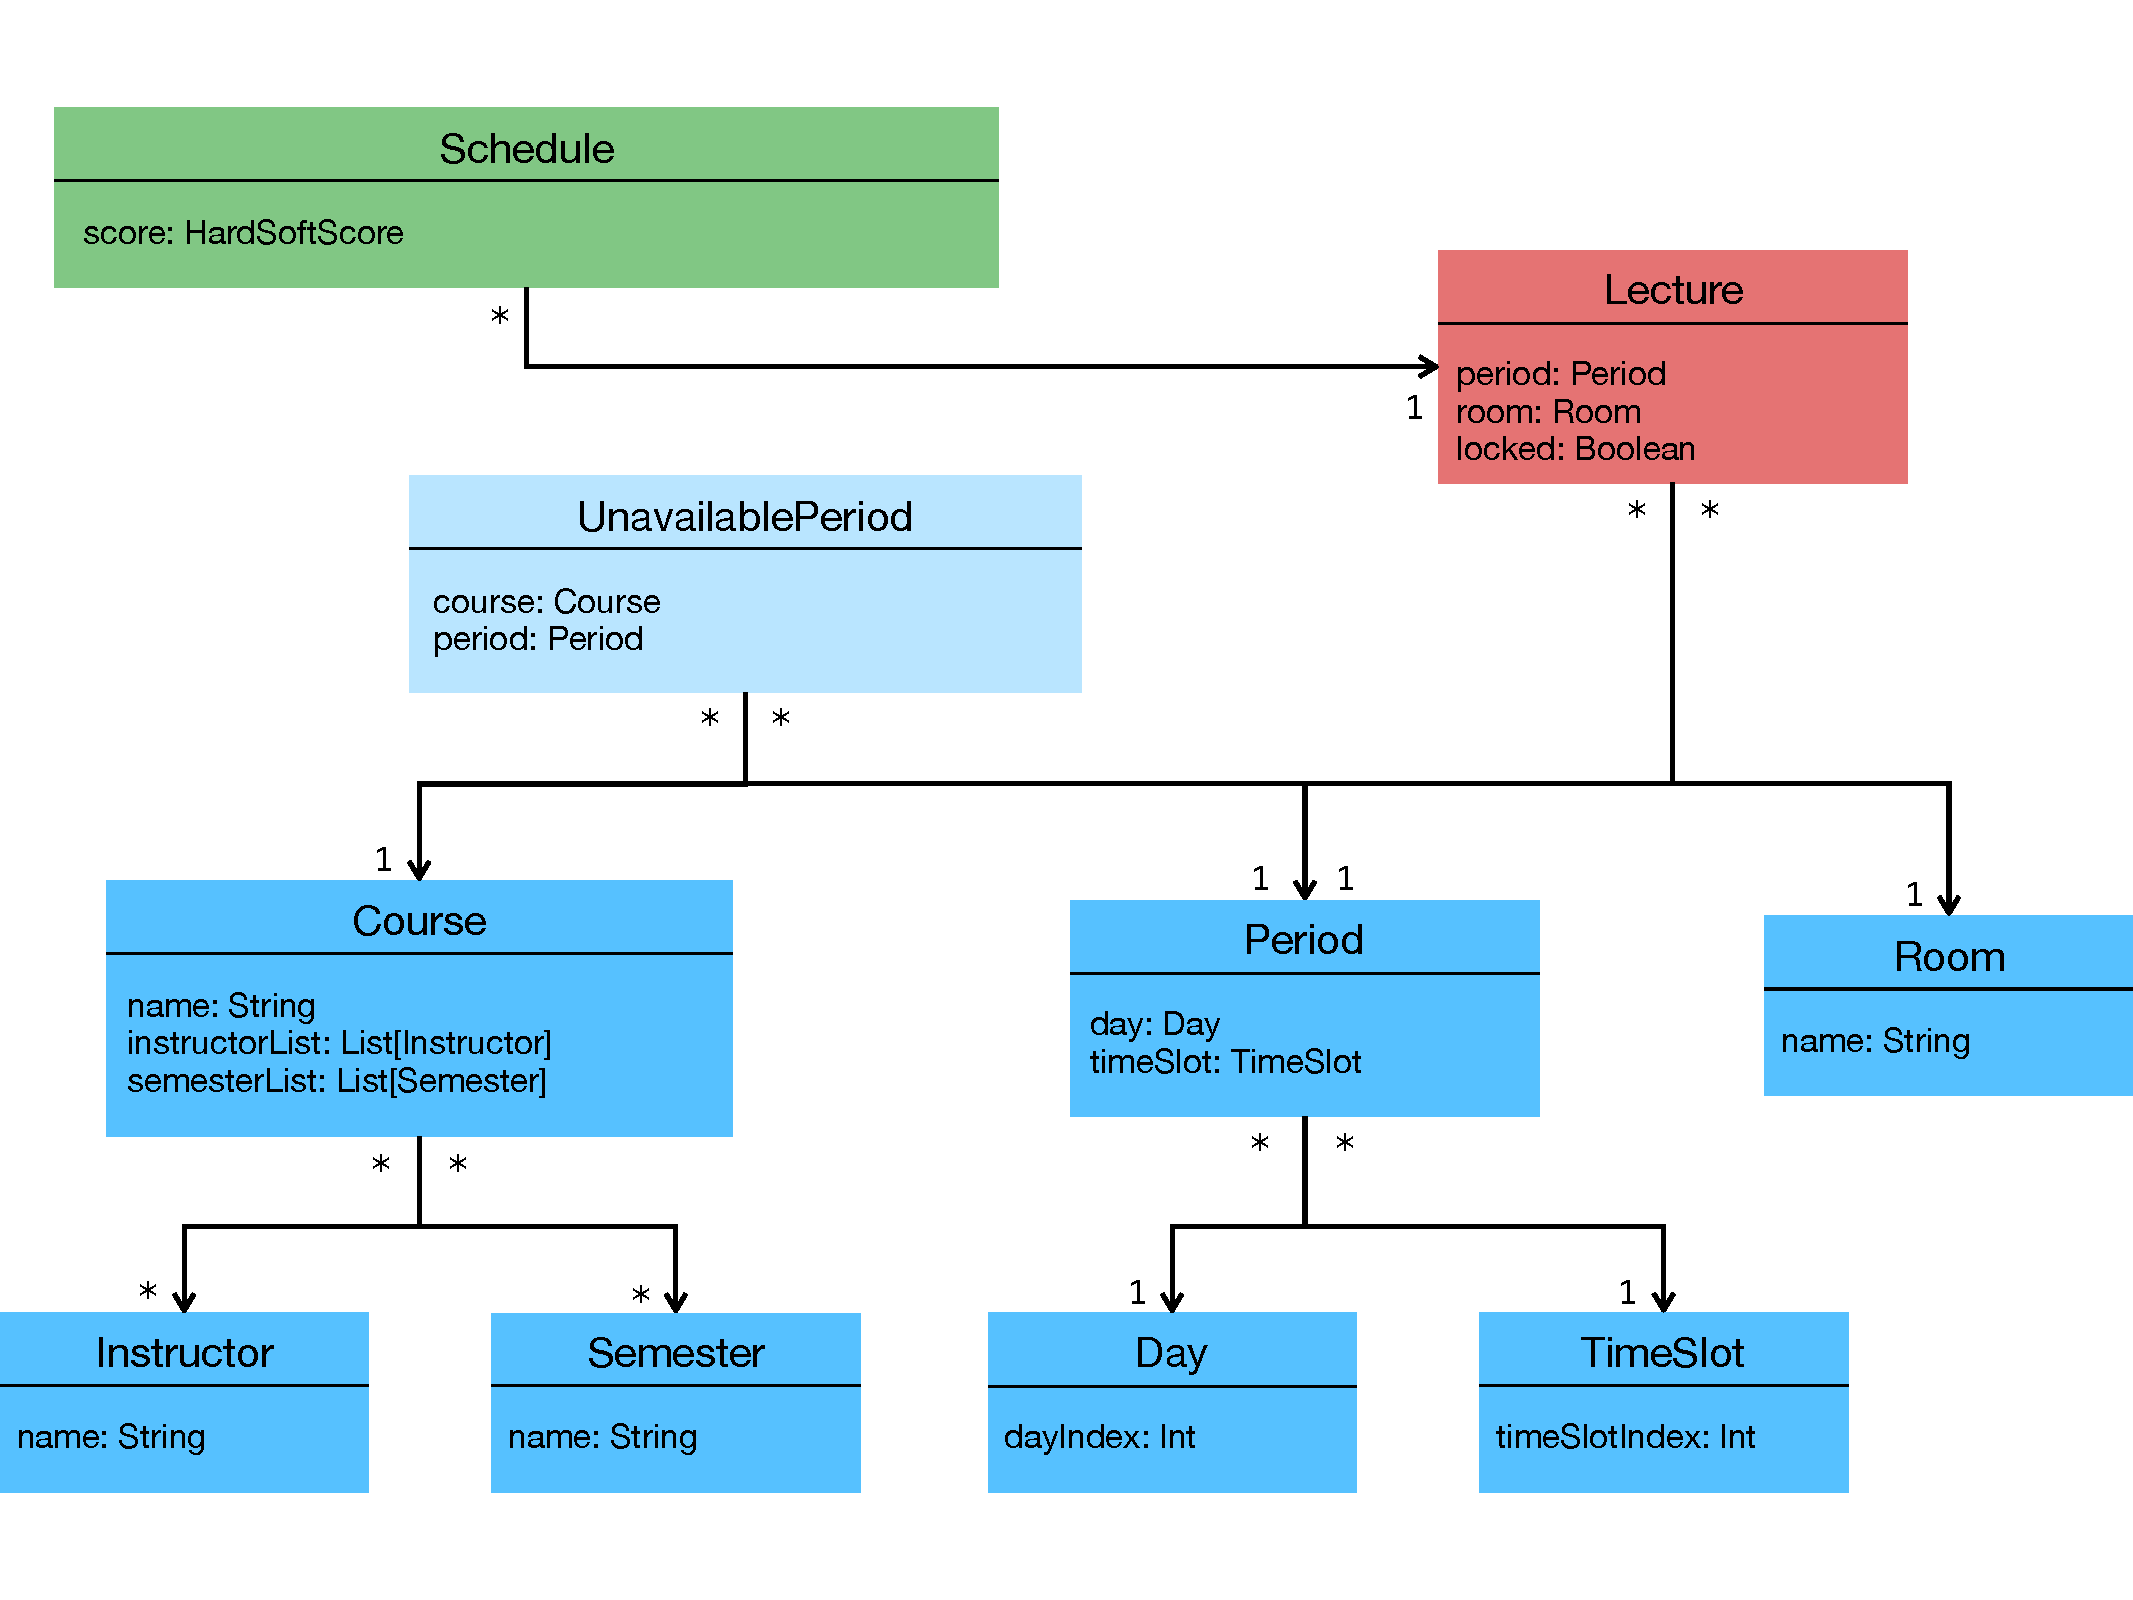
\includegraphics[width=\textwidth]{img/domainUML.pdf}
\caption{Class diagram of the domain model\label{fig:domainUML}}
\end{figure}
To know more about the inner workings of OptaPlanner, see appendix \ref{appendix:optaplanner}.

%_______________________________________________________________________________
\section{Constraints\label{sec:constraints}}
The constraints are of two kinds, hard constraints and soft constraints, as described in section \ref{sec:problem}.\par
As a rule, any solution that violates any hard constraint is unusable, since hard constraints model physical limitations (such as the impossibility for an instructor to teach two lectures at the same time).

%_______________________________________________________________________________
\section{Server and GraphQL API\label{sec:graphql}}

%_______________________________________________________________________________
\section{Web application UI\label{sec:web}}

%%%%%%%%%%%%%%%%%%%%%%%%%%%%%%%%%%%%%%%%%%%%%%%%%%%%%%%%%%%%%%%%%%%%%%%%%%%%%%%%
%%%%%%%%%%%%%%%%%%%%%%%%%%%%%%%%%%%%%%%%%%%%%%%%%%%%%%%%%%%%%%%%%%%%%%%%%%%%%%%%
\chapter{Conclusion}

%_______________________________________________________________________________
\section{Future work}

%%%%%%%%%%%%%%%%%%%%%%%%%%%%%%%%%%%%%%%%%%%%%%%%%%%%%%%%%%%%%%%%%%%%%%%%%%%%%%%%
%%%%%%%%%%%%%%%%%%%%%%%%%%%%%%%%%%%%%%%%%%%%%%%%%%%%%%%%%%%%%%%%%%%%%%%%%%%%%%%%
\appendix
\chapter{OptaPlanner\label{appendix:optaplanner}}
\chapter{GraphQL\label{appendix:graphql}}
This is the OptaPlanner appendix...

%%%%%%%%%%%%%%%%%%%%%%%%%%%%%%%%%%%%%%%%%%%%%%%%%%%%%%%%%%%%%%%%%%%%%%%%%%%%%%%%
%%%%%%%%%%%%%%%%%%%%%%%%%%%%%%%%%%%%%%%%%%%%%%%%%%%%%%%%%%%%%%%%%%%%%%%%%%%%%%%%
\bibliography{report}{}
\bibliographystyle{plain}

\end{document}
